\chapter{Results}
\label{ch:results}
The Kalman filter and controls algorithms discussed in this thesis were implemented in software on a PackBot and run in an open field with an uneven surface consisting of dirt, gravel and asphalt as seen in Figure \ref{fig:resultsTestArea}. This testing area is difficult for the robots to navigate because pitch, roll and elevation have significant changes and the loose dirt and gravel can cause the tracks to slip leading to erroneous encoder data. The environment in addition to routes that force the robot to change linear and angular velocities excites all the modes of the system model as well as some effects, such as track slip, which are not modeled at all and rigorously tests the estimation and control algorithms.

\begin{figure}[ht!]
	\centering
	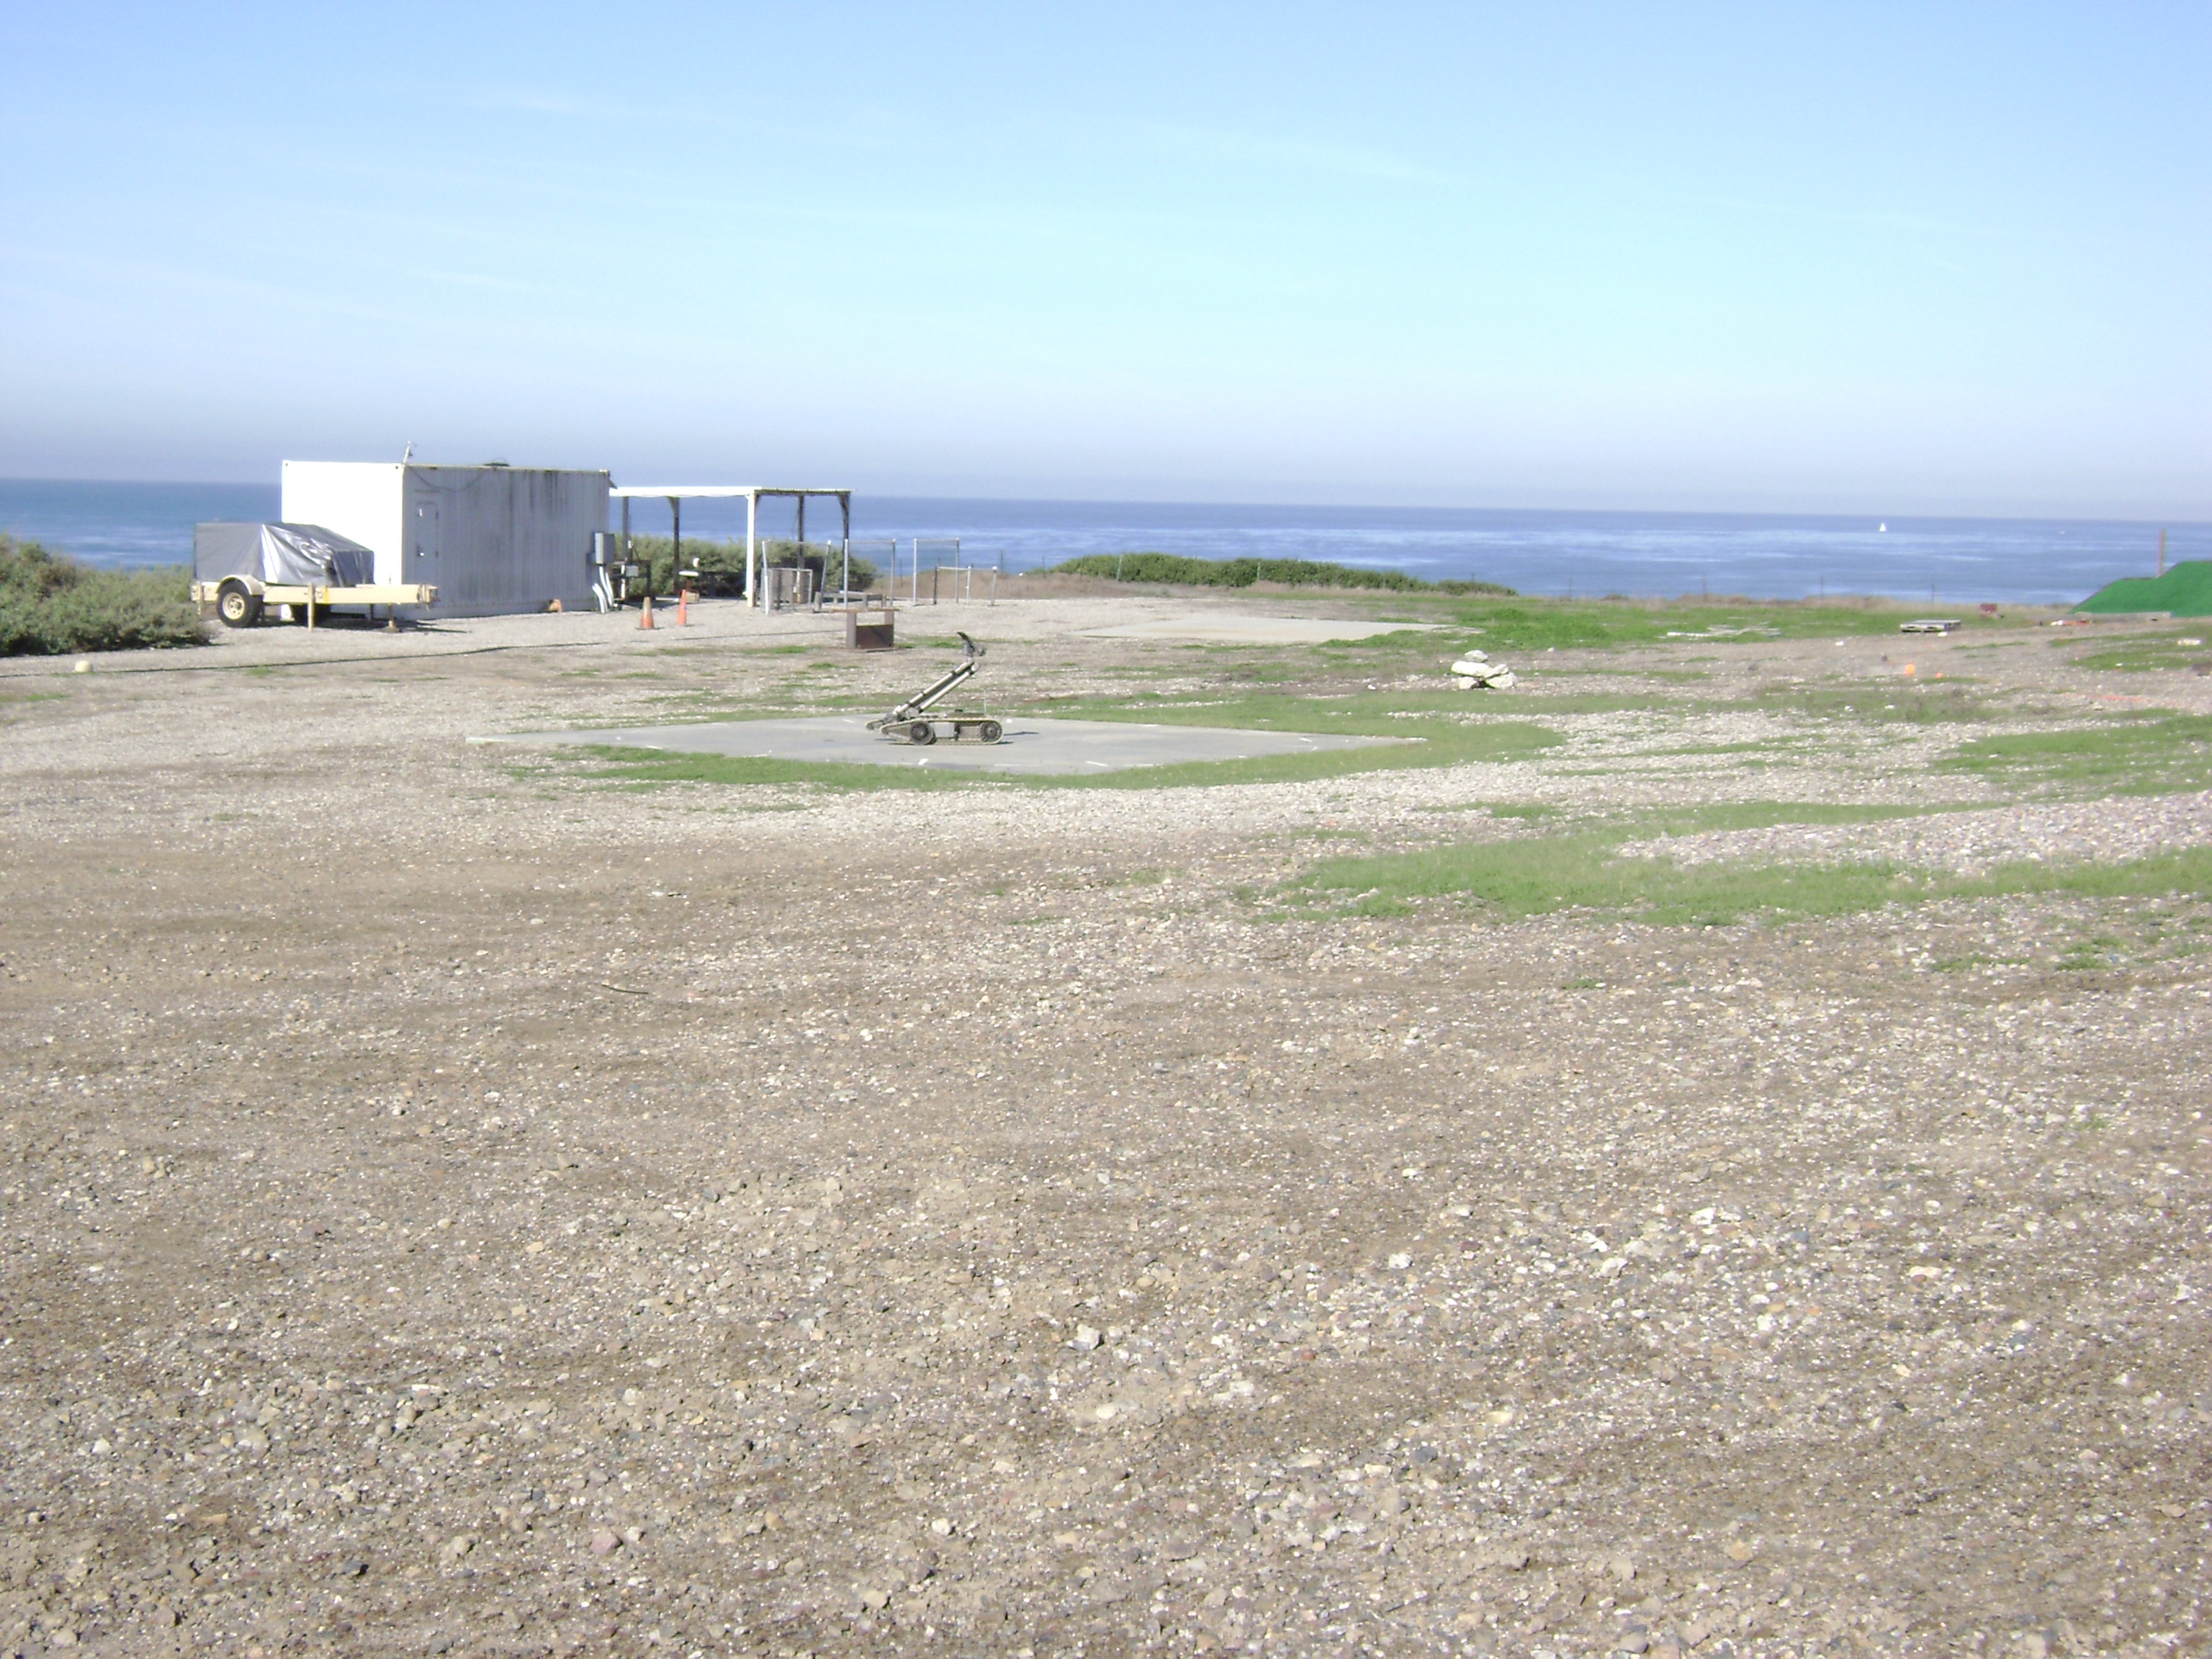
\includegraphics[width=.75\textwidth]{images/flightFieldTestArea}
	\caption{Robot Test Area}
	\label{fig:resultsTestArea}
\end{figure}

\section{Kalman Filter Results}
\label{sec:kfResults}
In Chapter \ref{ch:estimation} several aspects of the Kalman filter were modified with the goal of improving robot state estimation. Two metrics have been used to quantify the difference in performance of the Kalman filter after having made changes to the algorithm. Those metrics are the RMS error over the entire course and the amount of error in the position estimate before and after the robot runs a route where the percentage is the position error divided by the total amount of distance traveled over the route. The different changes that were tested were the baseline case, fixing the Kalman filter implementation bugs described in Chapter \ref{sec:kfBugs}, hand tuning the Kalman filter noise models and finally using noise models learned from the training algorithm from Chapter \ref{sec:kftrainingparams}. The results for Kalman filter performance are shown in Table \ref{tab:resultsKF}.

\begin{table}[ht!]
\caption{Kalman Filter Performance}
\small
\centering
\begin{tabular}{@{}llr@{}} \toprule
Stage                       & RMS Error (m)  & Return Error (\%) \\ \midrule
Baseline                    & 0              & 0                 \\
Fix KF Bugs                 & 0              & 0                 \\
Hand Tuned Noise Models     & 0              & 0                 \\
Training for Noise Models   & 0              & 0                 \\ \bottomrule
\end{tabular}
\label{tab:resultsKF}
\end{table}

\subsection{Kalman Filter Effects on Controller}
The model based and PID controllers were run with different stages of improvement in the Kalman filter. The results show that not only is the Kalman filter performance better but it can also be seen that the model based controller has much better performance when there are simulated obstacles along the route. In Figures \ref{fig:kfResults1} - \ref{fig:kfResults4} the same route was driven and the waypoints making up the route are shown on the overhead images. The red line is the Kalman filter position esimate, the blue line is raw GPS measurements and the green line is DPGS measurements.

The results of using the model based controller with original noise models is shown in Figure \ref{fig:kfResults1}. It can be seen that going from waypoint $4$ to waypoint $5$ the Kalman filter started to diverge significantly from the GPS measurements and the filter estimate snaps back to line up with the GPS measurements.

\begin{figure}[ht!]
	\centering
	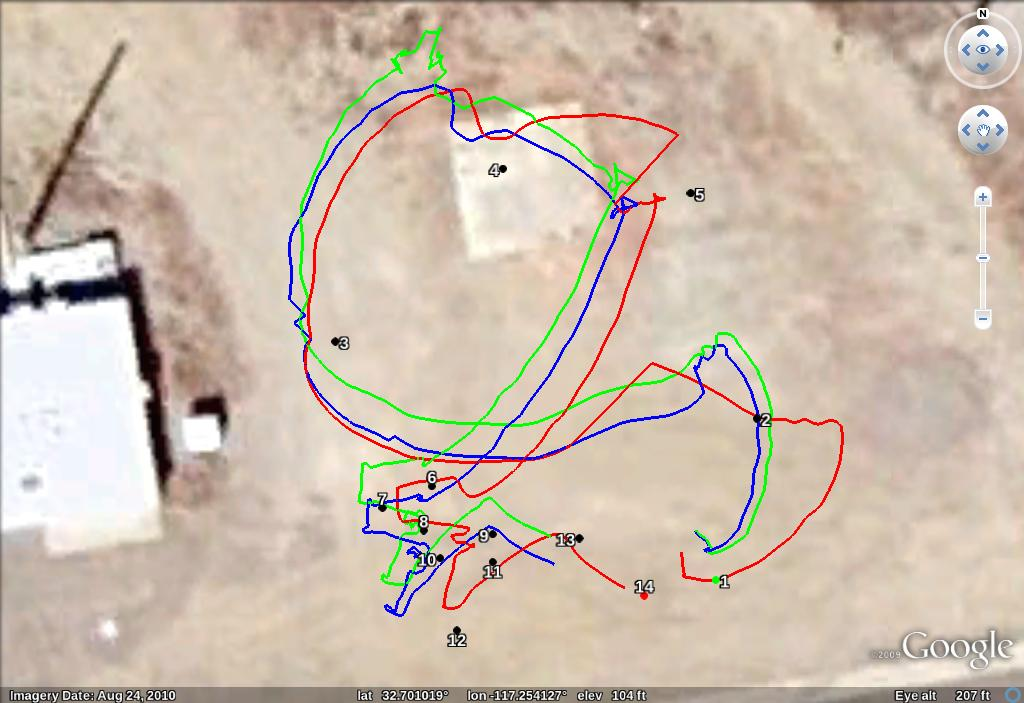
\includegraphics[width=.75\textwidth]{images/GE/20101203_1551_kf_lyapOrigQR}
	\caption{Model Based Controller with Original Noise Models}
	\label{fig:kfResults1}
\end{figure}

Running the model based controller with learned noise models resulted in the positions shown in Figure \ref{fig:kfResults2}. Here it can be seen that the Kalman filter position estimate is much closer to the GPS measurements for the entire route and that in certain places, such as near waypoint $4$ and between waypoint $6$ and waypoint $7$ the Kalman filter is able to remove discontinuities in the GPS position. Also, in the section of the route with waypoints close to each other to simulate navigation around obstacles the model based controller is able to drive through the waypoints.

\begin{figure}[ht!]
	\centering
	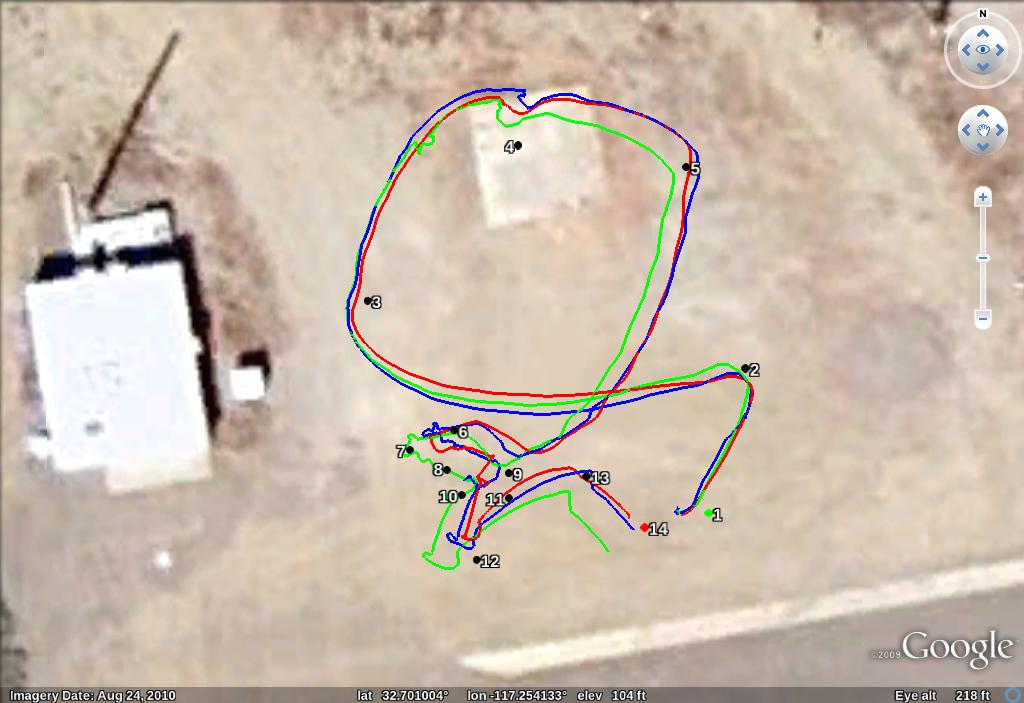
\includegraphics[width=.75\textwidth]{images/GE/20101203_1545_kf_lyapNewQR}
	\caption{Model Based Controller with Learned Noise Models}
	\label{fig:kfResults2}
\end{figure}

The PID controller with original noise models is shown in Figure \ref{fig:kfResults3}. Similar results are seen in regards to the Kalman filter position estimate snapping to the GPS measurements when significant divergence occurs between wayoint $2$ and waypoint $3$. The PID controller has trouble in the section of the route between waypoint $6$ and waypoint $12$ where the waypoints were set up close together to simulate obstacle along the route. In this section of the route the Kalman filter yaw estimate becomes very poor as the robot was driving in circles trying to reach the waypoints and as a result the Kalman filter position estimate diverges and would have snapped back to the GPS measurement if the route were not finished at waypoint $14$.

\begin{figure}[ht!]
	\centering
	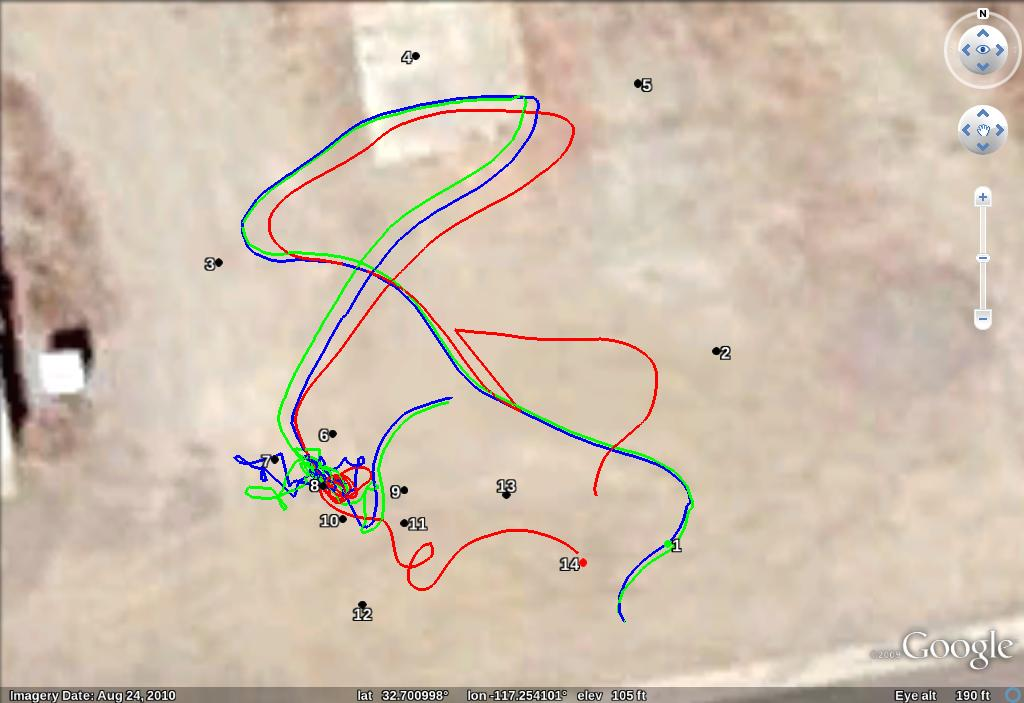
\includegraphics[width=.75\textwidth]{images/GE/20101203_1755_kf_pidOrigQR}
	\caption{PID Controller with Original Noise Models}
	\label{fig:kfResults3}
\end{figure}

The PID controller with learned noise models has similar trouble navigating the waypoints that are close together as seen in Figure \ref{fig:kfResults4}. However, with the learned noise models the Kalman filter position estimate stays much closer to the GPS measurements even when the robot is driving in circles. The improved position estimate is also indicative of an improved yaw estimate from the Kalman filter.

\begin{figure}[ht!]
	\centering
	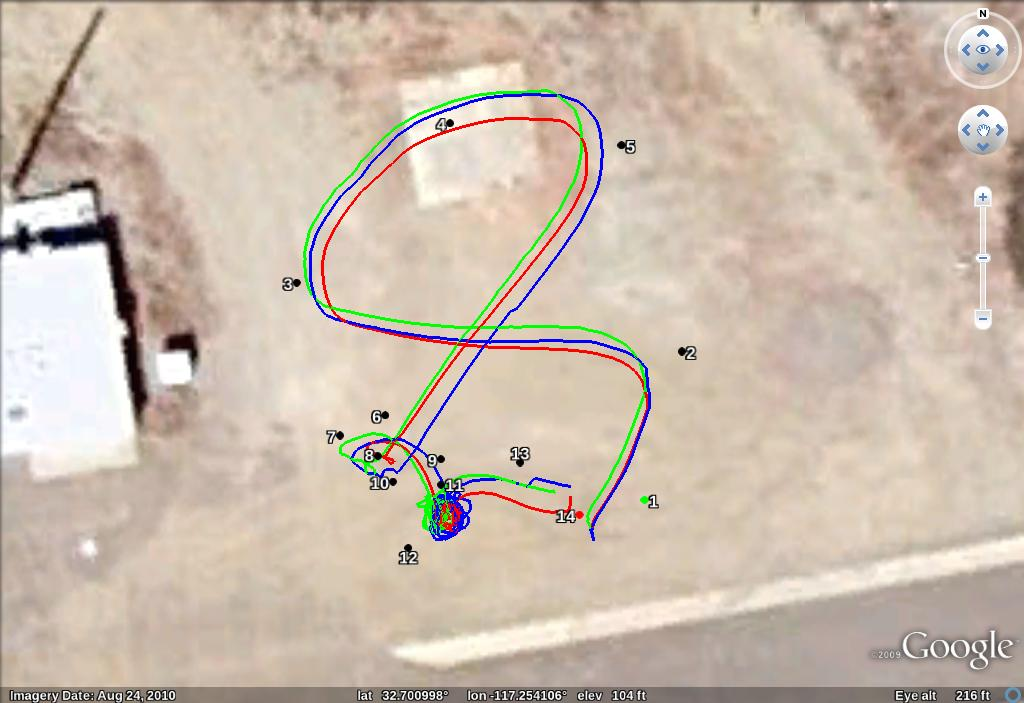
\includegraphics[width=.75\textwidth]{images/GE/20101203_1751_kf_pidNewQR}
	\caption{PID Controller with Learned Noise Models}
	\label{fig:kfResults4}
\end{figure}

\section{Model Based Controller Results}
\label{sec:lyapunovResults}
The control law derived in (\ref{eq:lyapunovControlLaw}) was tested in the previously described area in two different ways. The first set of results used a single set of gains and had the goal heading set to use the current heading of the robot so that $\theta^\star=\alpha$ as discussed in Chapter \ref{sec:lyapunovVariables}. Figure *** shows the actual position of the robot during navigation as well as the waypoints that defined the desired route.

Figures \ref{fig:resultsLyapunov1} - \ref{fig:resultsLyapunov4} shows how the linear and angular velocities changed over time as measured by the Kalman filter output. The gains used were $h=0.1$, $k=0.25$ and $\gamma=0.23$. A clear deceleration can be seen as the robot approaches each waypoint although the linear velocity does not go to zero until the final waypoint due to the use of the carrot in the path planner as discussed in Chapter \ref{sec:lyapunovVariables} for determing the error distance $e$. One of the consequences of using a model based controller is that a negative linear velocity was used after reaching the second waypoint and having the error angle $\alpha$ move towards the third waypoint which is rarely, if ever, encountered when using the original PID controller.

\begin{figure}[ht!]
	\centering
	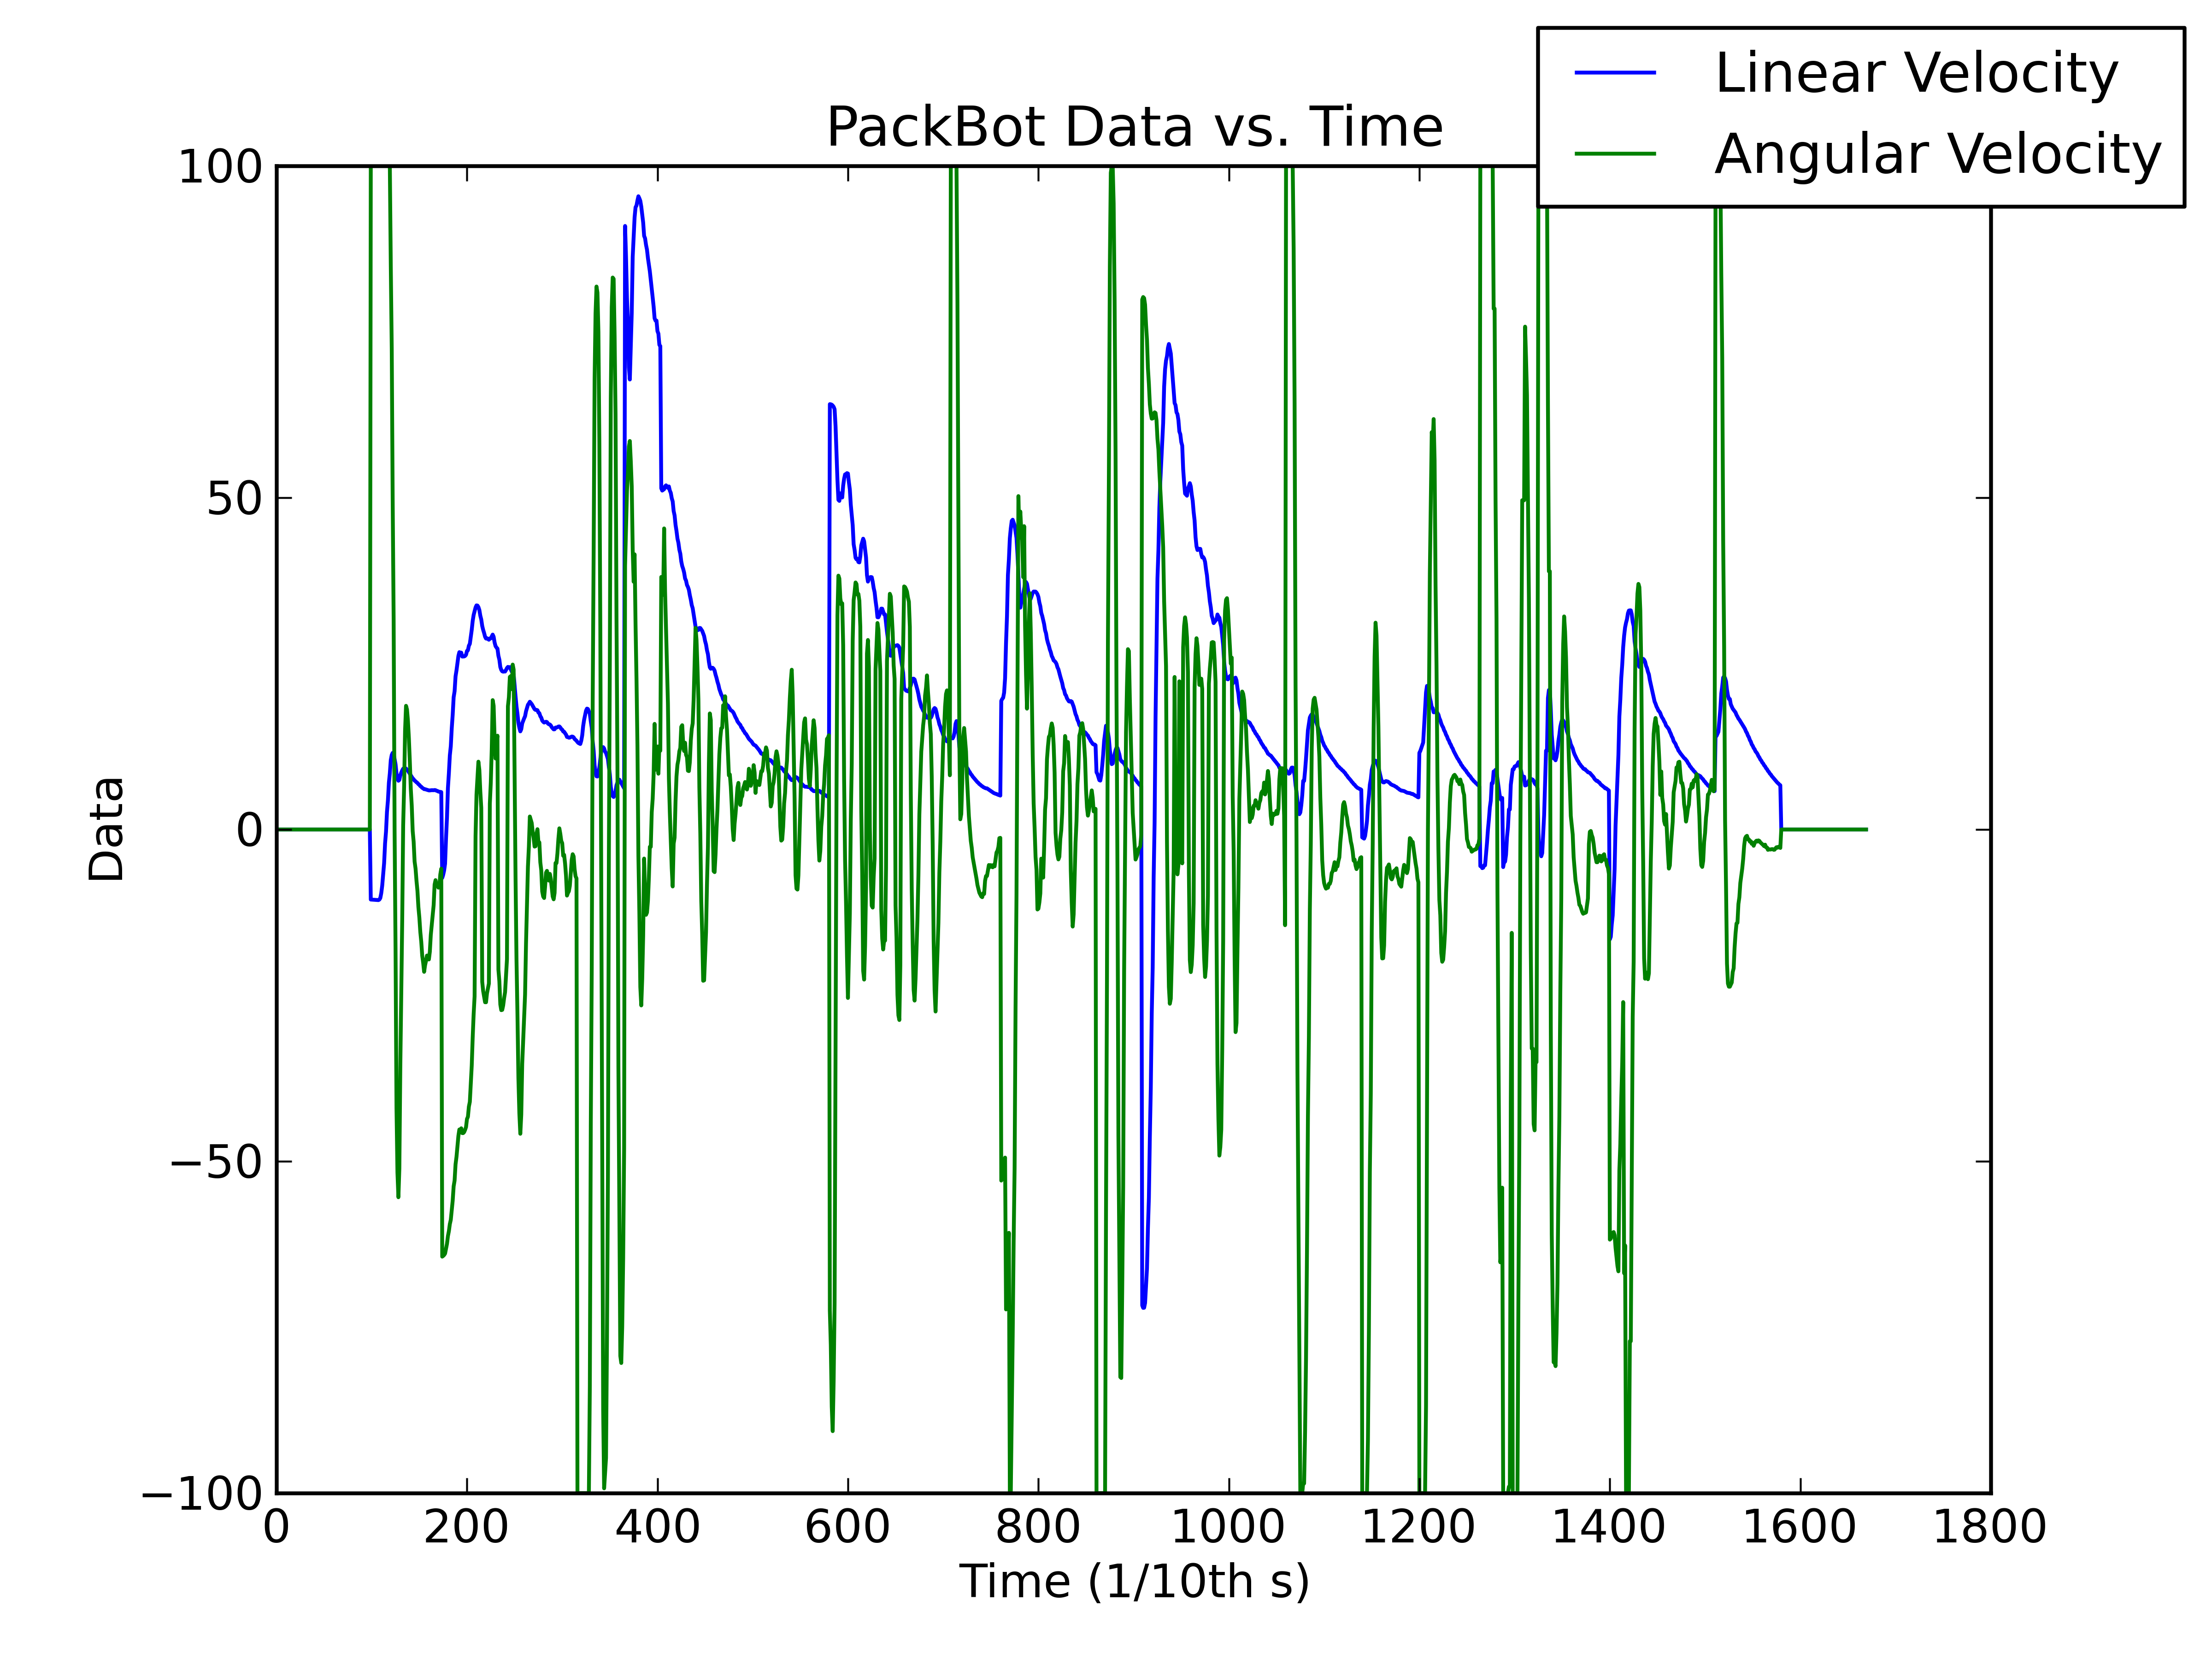
\includegraphics[width=.5\textwidth]{images/pbtx/20101203_1551_pbtxLyapOrigQR}
	\caption{Model Based Controller with Original Noise Models}
	\label{fig:resultsLyapunov1}
\end{figure}

\begin{figure}[ht!]
	\centering
	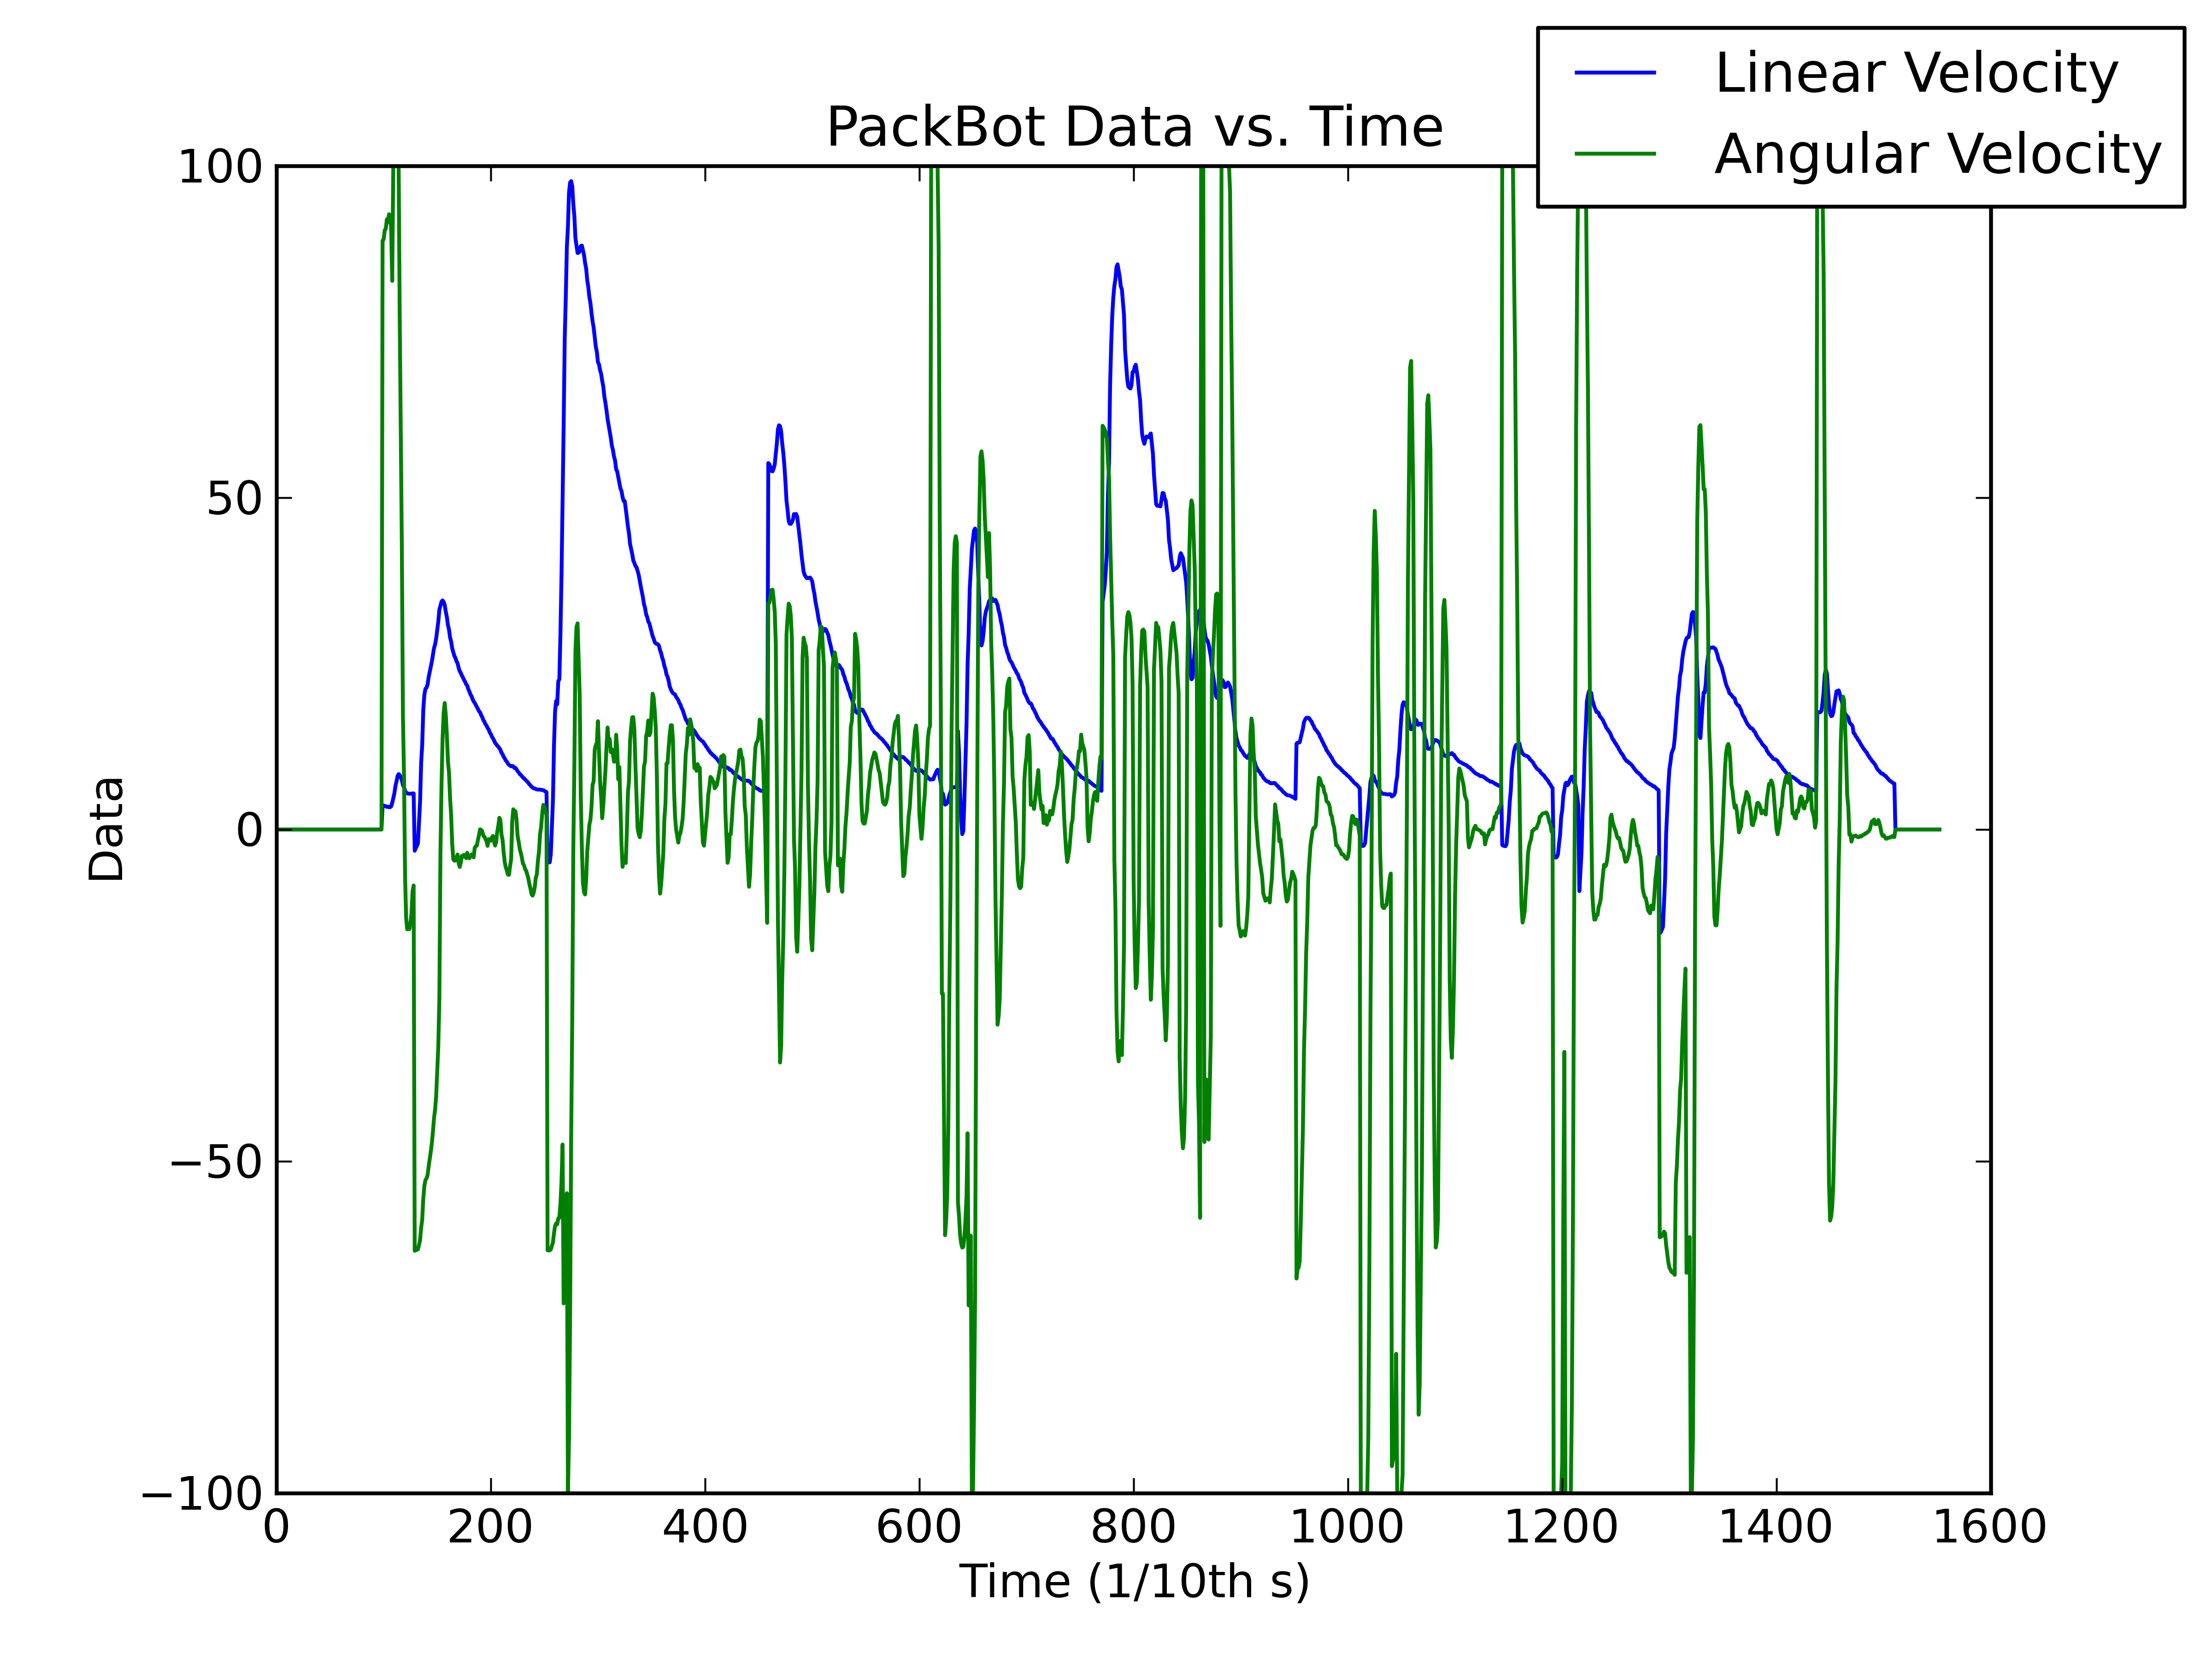
\includegraphics[width=.5\textwidth]{images/pbtx/20101203_1545_pbtxLyapNewQR}
	\caption{Model Based Controller with Learned Noise Models}
	\label{fig:resultsLyapunov2}
\end{figure}

\begin{figure}[ht!]
	\centering
	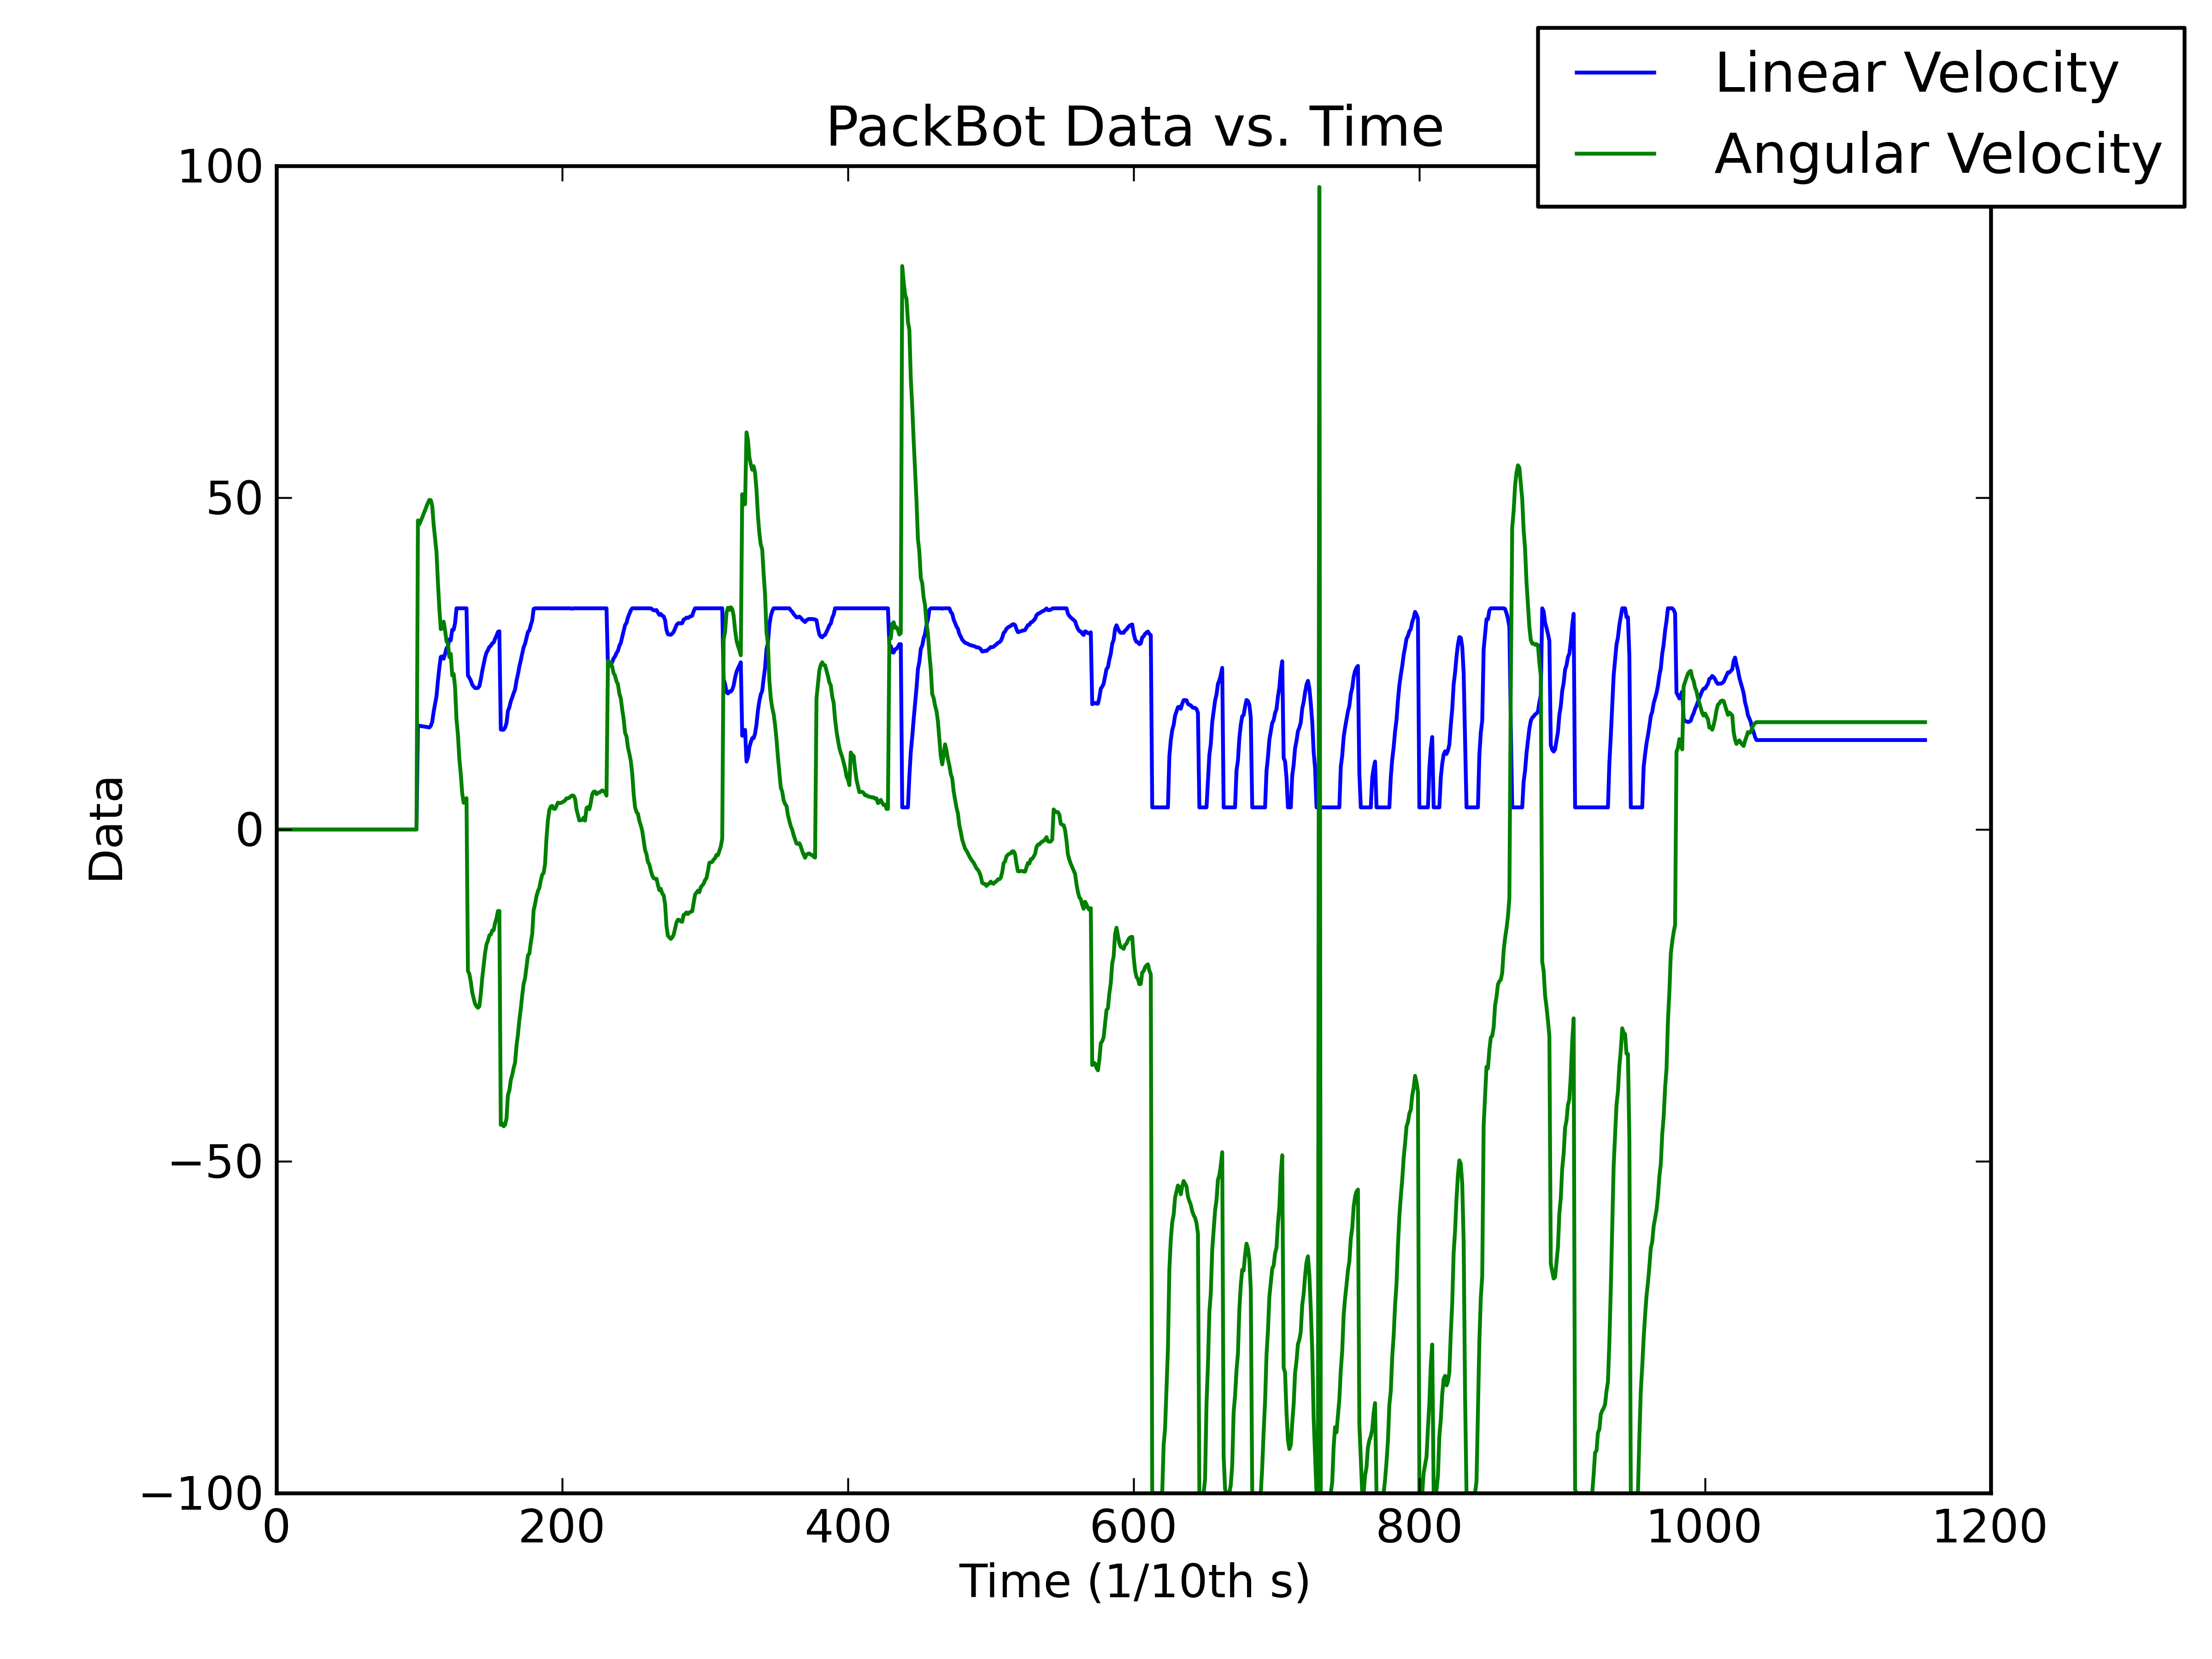
\includegraphics[width=.5\textwidth]{images/pbtx/20101203_1755_pbtxPidOrigQR}
	\caption{PID Controller with Original Noise Models}
	\label{fig:resultsLyapunov3}
\end{figure}

\begin{figure}[ht!]
	\centering
	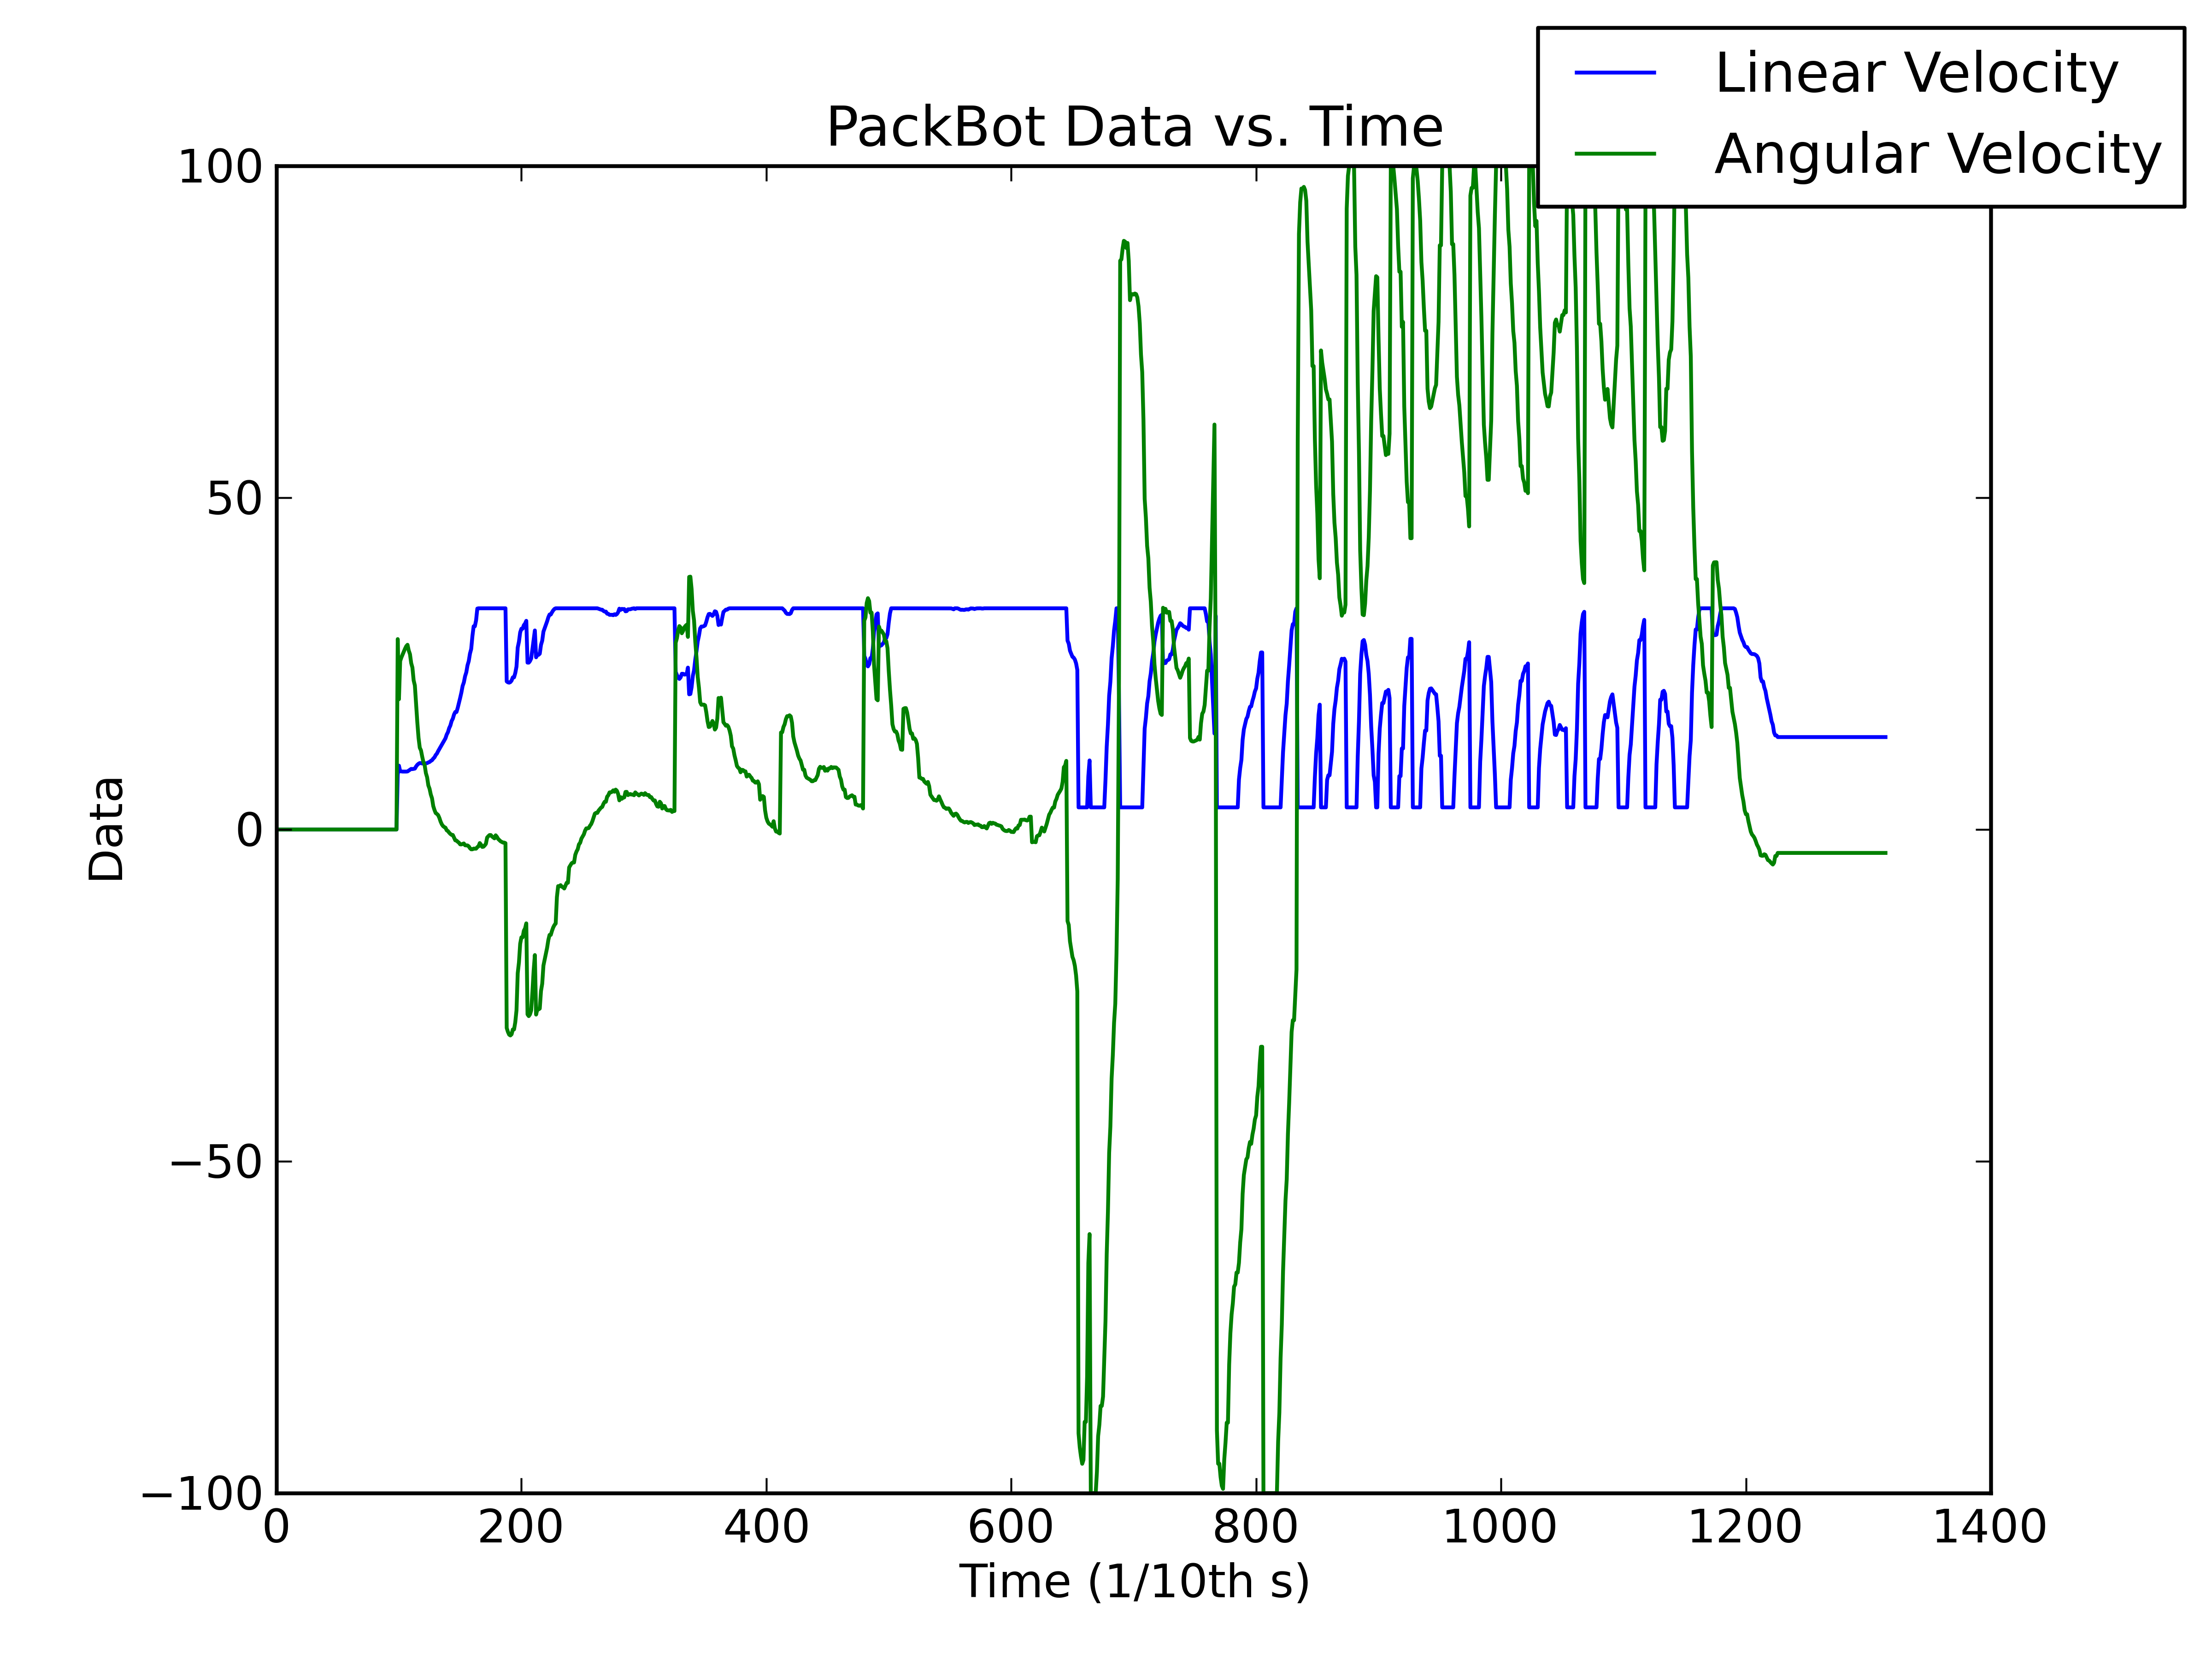
\includegraphics[width=.5\textwidth]{images/pbtx/20101203_1751_pbtxPidNewQR}
	\caption{PID Controller with Learned Noise Models}
	\label{fig:resultsLyapunov4}
\end{figure}

The process of selecting gains in Chapter \ref{sec:lyapunovTrajectoryConvergence} only applies as $(\alpha, \theta)\to(0,0)$ but says nothing about what happens when the angle errors are not small. Empirically it was determined that the gains $h=0.25$, $k=0.2$ and $\gamma=0.2$ worked well in creating smooth trajectories and later it was found that these gains cause $\zeta=1$ so that, when the angle errors are small, the system $A$ is critically damped although $\sigma>\gamma$ so the distance error converges faster than the angle errors. The best results occurred when the gains were set to $h=0.25$, $k=0.2$ and $\gamma=0.2$ \textit{until} the angle errors were $|\alpha|<0.5$ \textit{and} $|\theta|<0.5$ radians which leads to the linear approximation being valid and the gains were then changed to $h=1.1$, $k=0.42$ and $\gamma=0.2$. This second set of gains, used when the angle errors were small, are critically damped for the system $A$ since $\zeta=1$ and the angle errors converge faster than the distance error since $\sigma>\gamma$. The results of this adaptive gain scheme can be seen in Figures \ref{fig:resultsLyapunovPositionAdaptive} and \ref{fig:resultsLyapunovVelocitiesAdaptive}. Note that the goal heading, $\theta^\star$, was set to be the angle from the current waypoint to the next waypoint so that the robot would be pointing in the direction of the next waypoint when it reached the current waypoint. For the last waypoint in the route the goal heading used was $\theta^\star=\alpha$.

\begin{figure}[ht!]
	\centering
	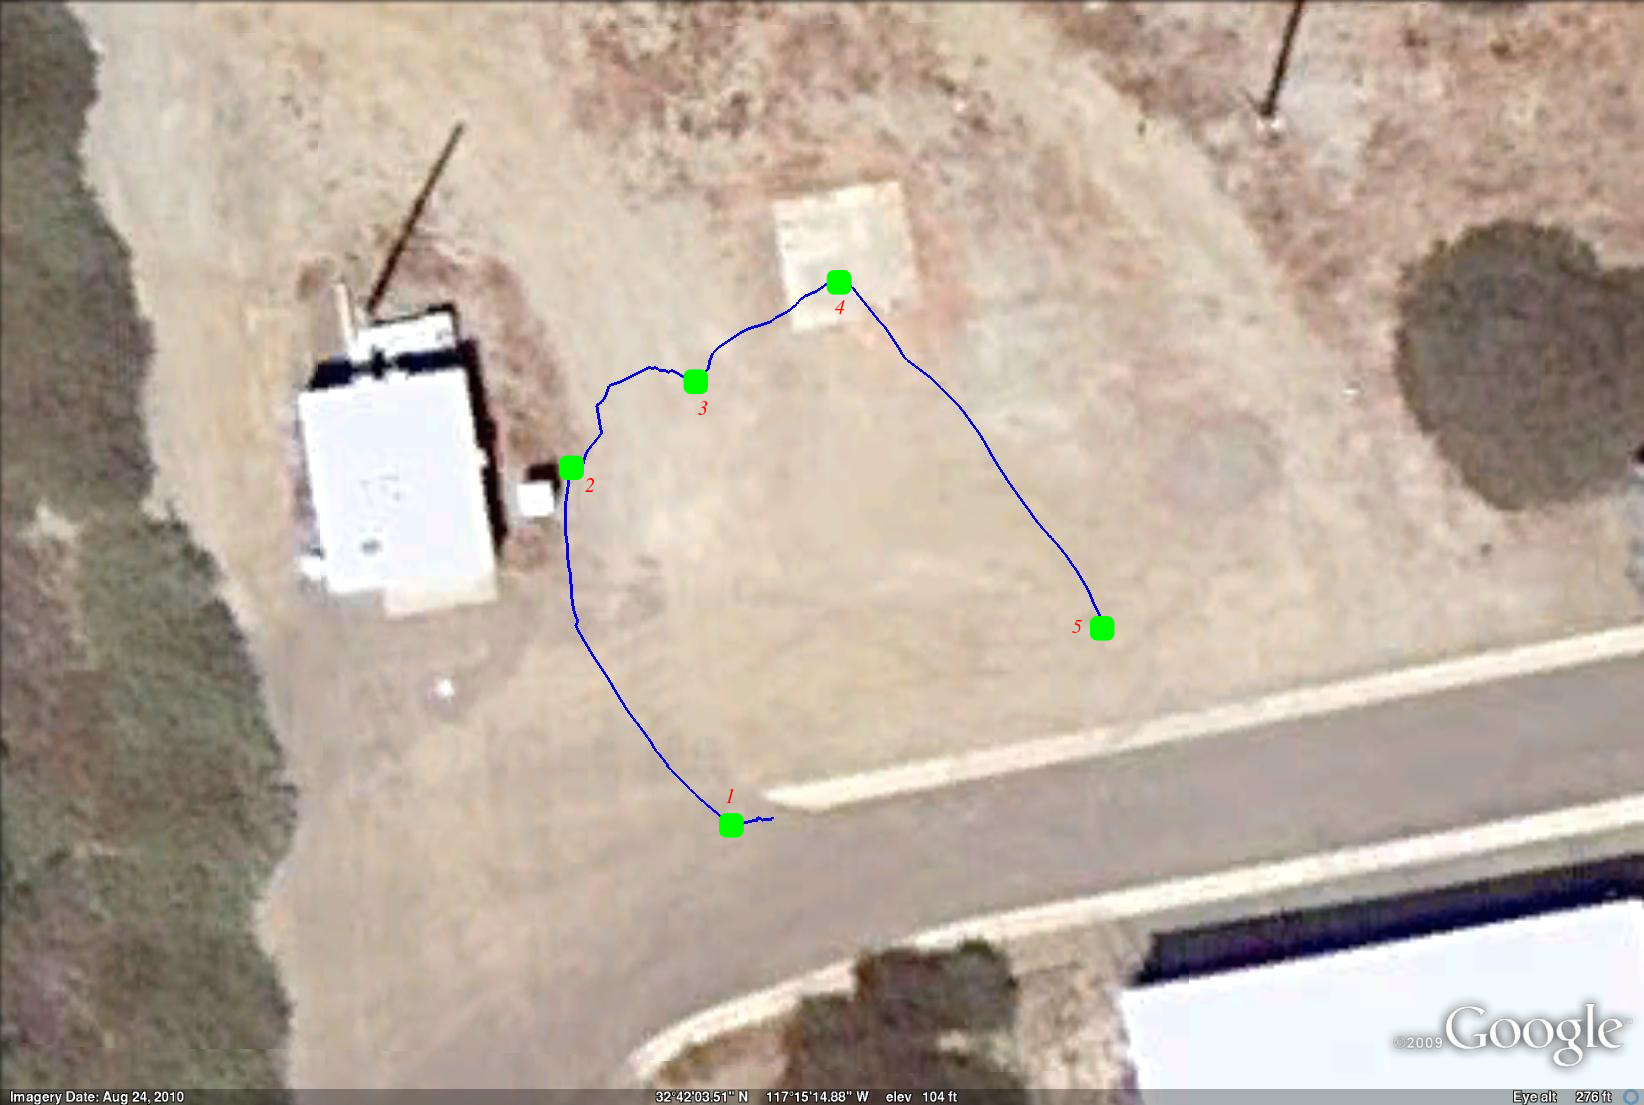
\includegraphics[width=.5\textwidth]{images/GE/20100929_1448_GE_KF_waypts}
	\caption{Robot Position using Adaptive Gain Scheme}
	\label{fig:resultsLyapunovPositionAdaptive}
\end{figure}

\begin{figure}[ht!]
	\centering
	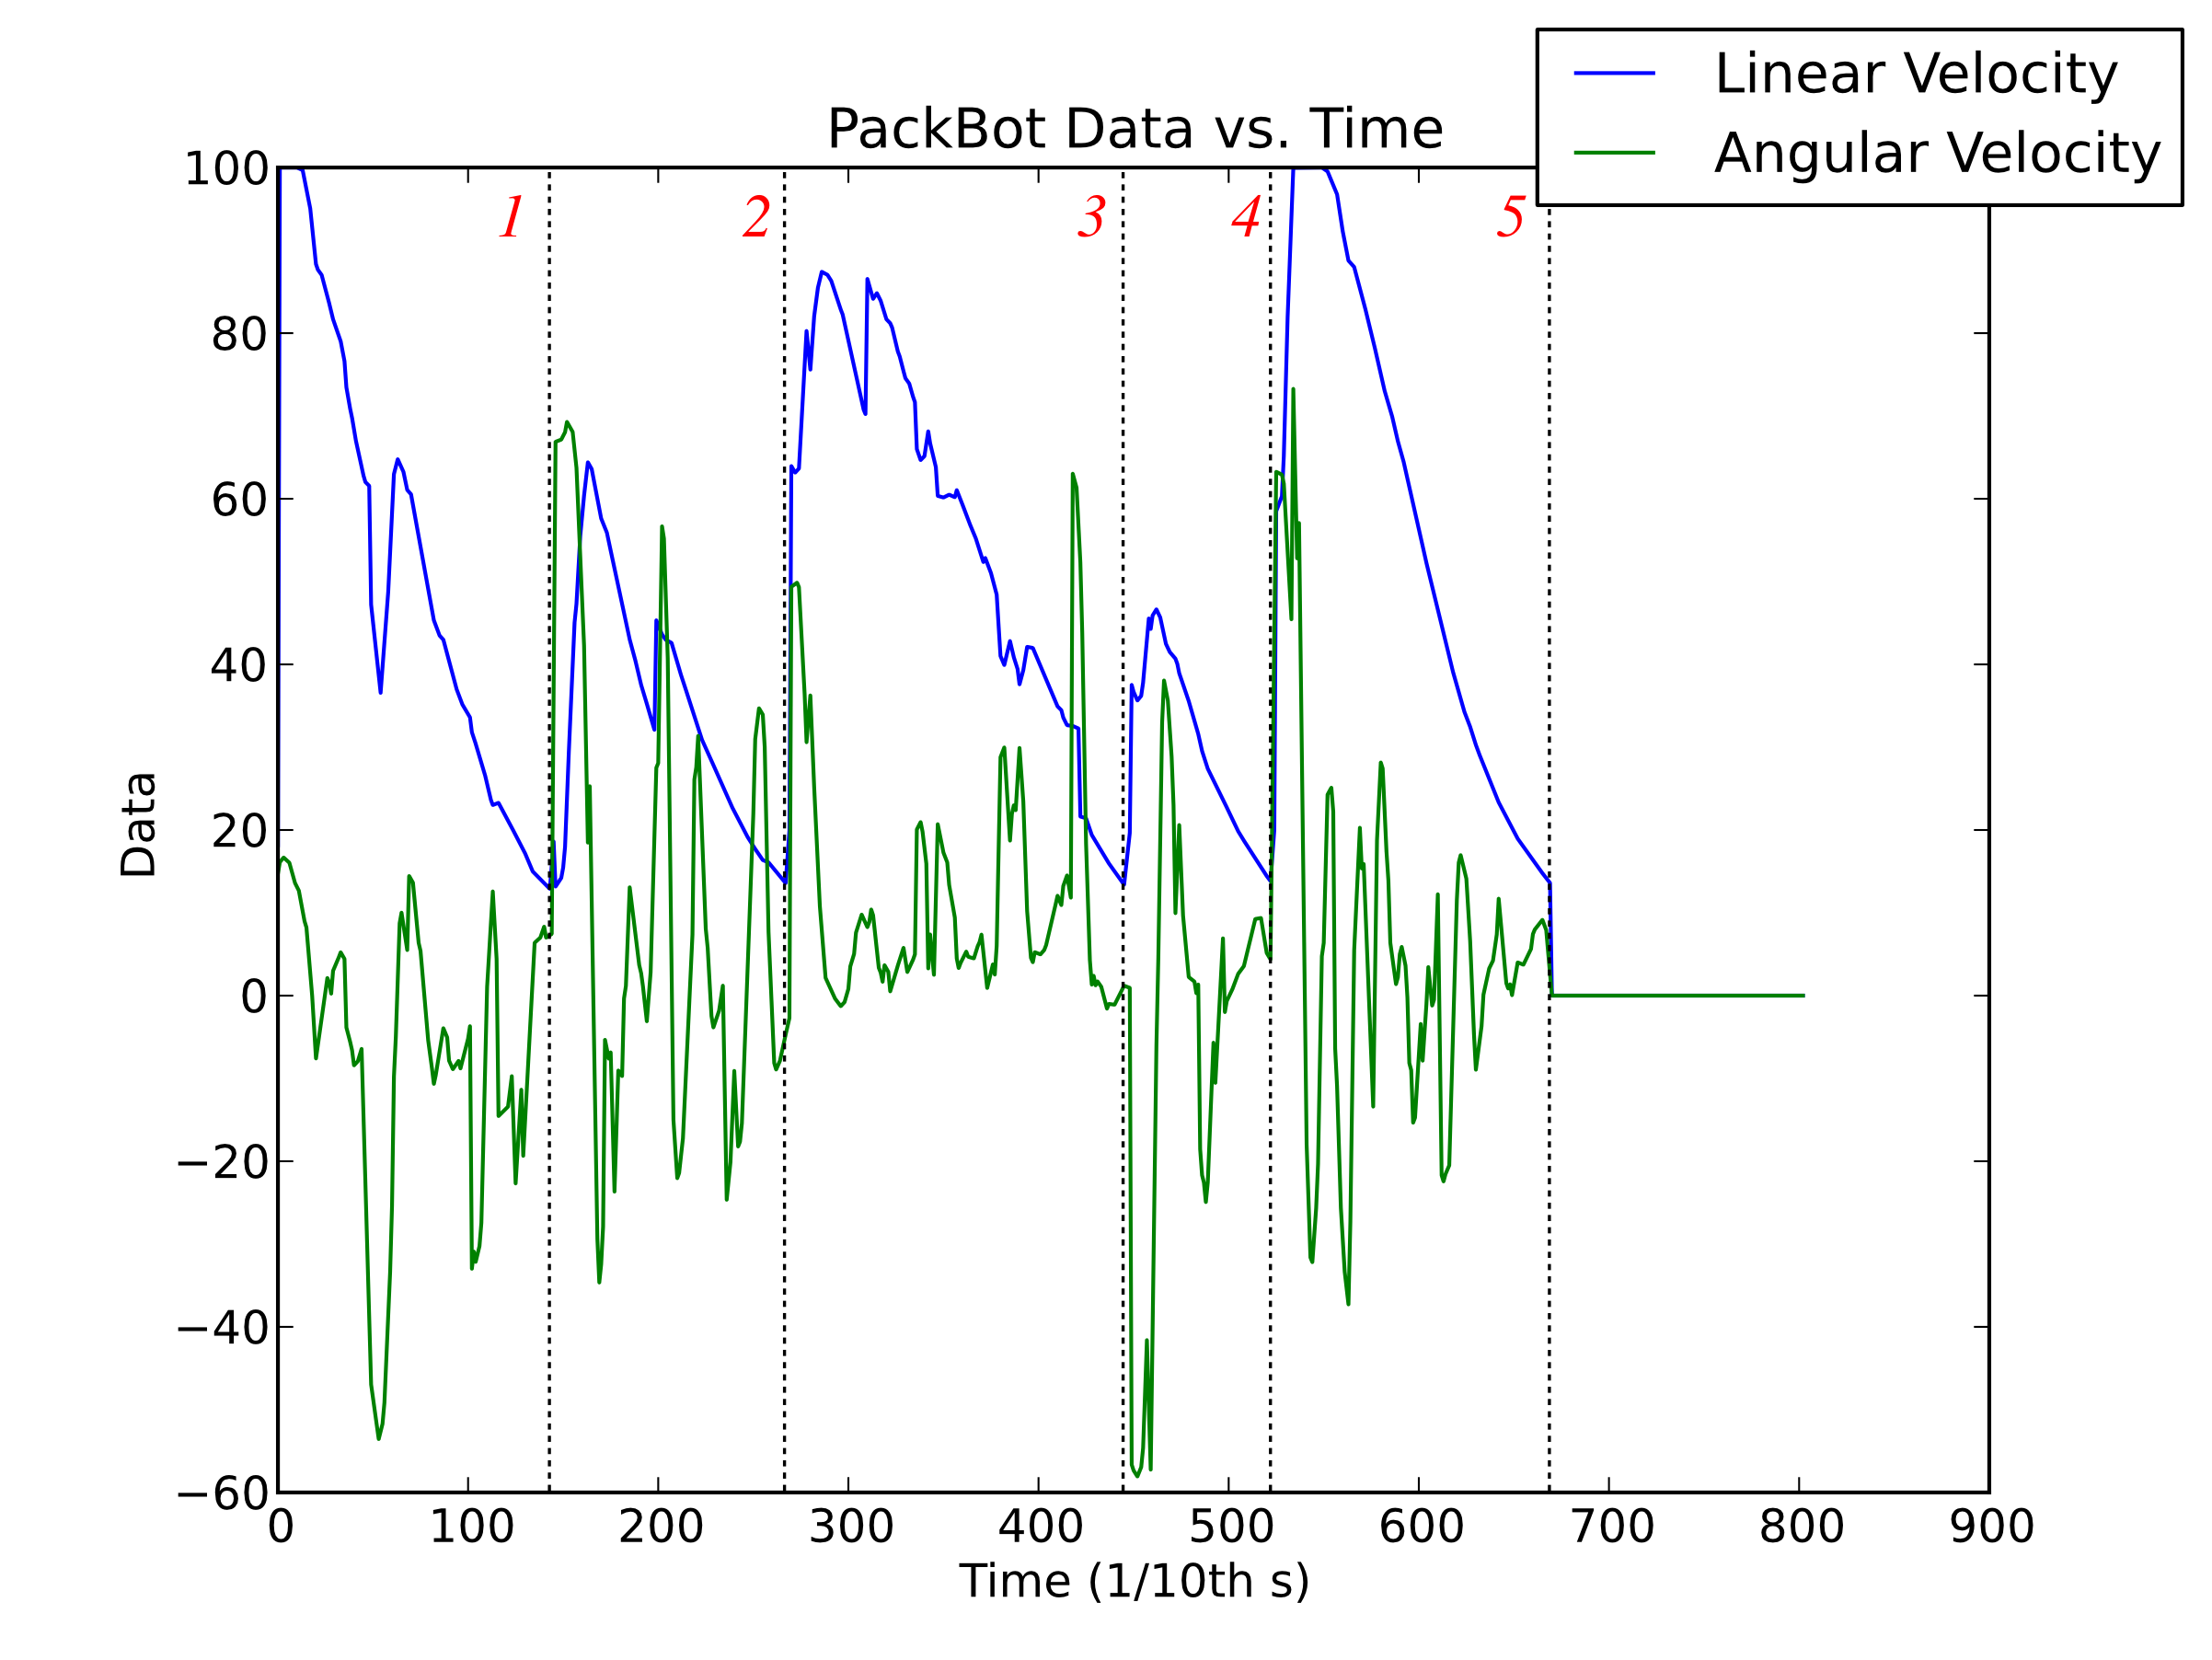
\includegraphics[width=.5\textwidth]{images/pbtx/20100929_1448_pbtx}
	\caption{Linear and Angular Velocities with Adaptive Gain Scheme}
	\label{fig:resultsLyapunovVelocitiesAdaptive}
\end{figure}

\subsection{Controller Comparison}
\label{sec:controllerComparison}
For both PID (Chapter \ref{sec:pid}, Table \ref{tab:PIDGainEffects}) and the model based controller (Chapter \ref{sec:lyapunovTrajectoryConvergence}) gains have to be selected, the difference being that stability is the goal when selecting PID gains whereas stability is guaranteed with the model based controller. More advanced behaviors such as three point turns are a consequence of the control law in (\ref{eq:lyapunovControlLaw}) derived using a kinematic model of the robot. The other very large difference between the controllers is that a table of gains must be tuned for the PID controller to work at varying linear velocities but the model based controller works very well at different linear and angular velocities. Also, when properties of the robot such as mass are changed by using different payloads for the system the entire table of PID gains must be retuned while, at most, one set of gains must be retuned for the model based controller. This last benefit of the model based controller makes it very appealing to use in fielded systems since it reduces the amount of maintenance and effort required to keep the robot in working condition. The model based controller will also allow for improved navigation performance near obstacles which leads directly to improved autonomy for the robot.

Many different controller configurations are possible based on varying the gains used and the calculation of the desired heading at waypoints. The tested configurations included:
\begin{enumerate}
\item PID with best available gains,
\item Fuzzy logic with best available rules,
\item Model based with $\theta^\star$ set as angle from current waypoint to next waypoint with gains set to minimize distance error before angle errors ($\gamma = $, $h = $, $k = $),
\item Model based with $\theta^\star$ set as angle from previous waypoint to current waypoint with gains set to minimize distance error before angle errors ($\gamma = $, $h = $, $k = $),
\item Model based with $\theta^\star$ set as angle from current waypoint to next waypoint with gains set to minimize angle errors before distance error ($\gamma = $, $h = $, $k = $),
\item Model based with $\theta^\star$ set as angle from previous waypoint to current waypoint with gains set to minimize angle errors before distance error ($\gamma = $, $h = $, $k = $),
\item Model based with $\theta^\star$ set as angle from current waypoint to next waypoint with gains set to minimize distance error before $\alpha$ before $\theta$ ($\gamma = $, $h = $, $k = $),
\item Model based with $\theta^\star$ set as angle from previous waypoint to current waypoint with gains set to minimize distance error before $\alpha$ before $\theta$ ($\gamma = $, $h = $, $k = $),
\item Model based with parking behavior turned on and gains set to have angle errors converge at the same rate and faster than the distance error converges ($\gamma = 0.25$, $h = 1.1$, $k = 2\gamma\sqrt{h}$).
\end{enumerate}
Note that in all cases for the model based controller the desired goal heading $\theta^\star$ for the final waypoint was set to be the angle from the previous waypoint to the last waypoint.

Each controller configuration was run on several courses that test specific behaviors such as
\begin{itemize}
\item allowing for maximum velocities to be sustained with large amounts of open space on the route by having long path segments shown in Figure ***,
\item short path segments between waypoints to simulate obstacles along the route shown in Figure ***,
\item a mixture of long and short path segments shown in Figure ***.
\end{itemize}

The results using the different setups described are shown for the different routes in Tables \ref{tab:resultsControllersOpenSpace} - \ref{tab:resultsControllersMixed} where the metrics used to compare the controller performance are
\begin{itemize}
\item the time required to complete the course,
\item the average cross track error during the course to show whether the robot followed a straight line between waypoints which is important when obstacles are in the area and not important when large amounts of open space are available for navigation (although some operators become nervous when the robot trajectory has large curvature and deviates from a straight line path even if open space is available),
\item the maximum velocity achieved by the robot during the course,
\item the number of times that the robot stops where a stop is defined as the robot having a velocity that drops below a small velocity.
\end{itemize}
Note that for the model based controller in driving mode values of $(\lambda, \epsilon)$ to control the extension of the distance error were $(???,???)$ for the open space route, $(???,???)$ for the obstacle route and $(???,???)$ for the mixed route and were determined empirically.

\begin{table}[ht!]
\caption{Controller Comparison on Open Space Route}
\small
\centering
\begin{tabular}{@{}llllr@{}} \toprule
Setup & Time (s) & Cross Track Error (m) & Max Velocity (m/s) & \# Stops \\ \midrule
1     & 0        & 0                     & 0                  & 0        \\
2     & 0        & 0                     & 0                  & 0        \\
3     & 0        & 0                     & 0                  & 0        \\
4     & 0        & 0                     & 0                  & 0        \\
5     & 0        & 0                     & 0                  & 0        \\
6     & 0        & 0                     & 0                  & 0        \\
7     & 0        & 0                     & 0                  & 0        \\
8     & 0        & 0                     & 0                  & 0        \\
9     & 0        & 0                     & 0                  & 0        \\ \bottomrule
\end{tabular}
\label{tab:resultsControllersOpenSpace}
\end{table}

\begin{table}[ht!]
\caption{Controller Comparison on Simulated Obstacle Route}
\small
\centering
\begin{tabular}{@{}llllr@{}} \toprule
Setup & Time (s) & Cross Track Error (m) & Max Velocity (m/s) & \# Stops \\ \midrule
1     & 0        & 0                     & 0                  & 0        \\
2     & 0        & 0                     & 0                  & 0        \\
3     & 0        & 0                     & 0                  & 0        \\
4     & 0        & 0                     & 0                  & 0        \\
5     & 0        & 0                     & 0                  & 0        \\
6     & 0        & 0                     & 0                  & 0        \\
7     & 0        & 0                     & 0                  & 0        \\
8     & 0        & 0                     & 0                  & 0        \\
9     & 0        & 0                     & 0                  & 0        \\ \bottomrule
\end{tabular}
\label{tab:resultsControllersObstacles}
\end{table}

\begin{table}[ht!]
\caption{Controller Comparison on Mixed Route}
\small
\centering
\begin{tabular}{@{}llllr@{}} \toprule
Setup & Time (s) & Cross Track Error (m) & Max Velocity (m/s) & \# Stops \\ \midrule
1     & 0        & 0                     & 0                  & 0        \\
2     & 0        & 0                     & 0                  & 0        \\
3     & 0        & 0                     & 0                  & 0        \\
4     & 0        & 0                     & 0                  & 0        \\
5     & 0        & 0                     & 0                  & 0        \\
6     & 0        & 0                     & 0                  & 0        \\
7     & 0        & 0                     & 0                  & 0        \\
8     & 0        & 0                     & 0                  & 0        \\
9     & 0        & 0                     & 0                  & 0        \\ \bottomrule
\end{tabular}
\label{tab:resultsControllersMixed}
\end{table}
